\documentclass[10pt,a4paper]{article}
\usepackage[utf8]{inputenc}
\usepackage[spanish, mexico]{babel}
\usepackage{listingsutf8}
\usepackage{color}
\usepackage{amsmath}
\usepackage{booktabs}
\usepackage{subcaption}
\usepackage{graphicx}
\usepackage{multicol} 
\usepackage{float}
\usepackage{wasysym}
\definecolor{codegreen}{rgb}{0,0.6,0}
\definecolor{codegray}{rgb}{0.5,0.5,0.5}
\definecolor{codepurple}{rgb}{0.58,0,0.82}
\definecolor{backcolour}{rgb}{0.95,0.95,0.92}
\usepackage[top=2cm,bottom=3cm,left=3cm,right=3cm]{geometry}
\setlength{\parskip}{\baselineskip} 

\begin{document}

\setlength{\unitlength}{1cm}
\thispagestyle{empty}
\begin{picture}(18,4)
\put(0,0.2){\includegraphics[scale=.2]{UNAM.jpg}}
\put(11.5,0){\includegraphics[scale=.5]{fc.png}}
\end{picture}
\begin{center}
\textbf{{\LARGE Universidad Nacional Autónoma de México}\\[1cm]
{\LARGE Facultad de Ciencias}}\\[1.8cm]
{\LARGE Práctica 13: Ondas estacionarias en una cuerda}\\[1.2cm]
\end{center}
\vspace{.7 cm}
\begin{flushleft}{\Large 14 de Noviembre de 2019 }\\[1 cm]
\end{flushleft}
\begin{flushright}{\Large{\underline{\textcolor{black}{López Cruz Ángel Jikmé}}}}\\[0.78cm]
\end{flushright}
\begin{flushright}{\Large{\underline{\textcolor{black}{López Velasco Juan Manuel}}}}\\[0.78cm]

\begin{flushright}{\Large{\underline{\textcolor{black}{Robledo Ibarra Emiliano}}}}\\[1 cm]
\end{flushright}\end{flushright}
\begin{center}
{\Large Profesor: Luis Quintanar Robles }\\[0.4cm]
{\Large Ayudante: Luis Enrique Quintanar Cortés }\\[1 cm]
\end{center}
RESUMEN:
Esta práctica tuvo como objetivo encontrar la relación entre las tensiones a las cuales se somete una cuerda, la cual se hace vibrar de modo que se genere un patrón de ondas estacionarias en ella y la frecuencia (a la que se hace vibrar la cuerda) necesaria para generar ciertas semilongitudes de onda. Para ello se midieron distintas tensiones bajo la misma longitud de la cuerda $L= (203.00\pm0.05) cm$. Se midieron las semilongitudes de onda producidas al someter a la cuerda a diferentes frecuencias, es decir, distintos patrones de ondas estacionarias, se relacionó la frecuencia y las semilongitudes por lo cual se obtuvo una relación  lineal entre dichas variables, notando que las pendientes eran distintas al cambiar la tensión se propuso una posible relación entre la tensión y las pendientes obtenidas. Se encontró dicha relación inversamente proporcional, por lo tanto las pendientes se obtuvieron en función de la tensión, lo que permitió generalizar la relación entre frecuencias y semilongitudes, se obtuvo la siguiente relación $n=(-0.0073 \pm 0.0008)TF + (0.083 \pm 0.003)F$ siendo $n$ el número de semilongitudes, $T$ la tensión en Newtons y $F$ la frecuencia del generador.
\normalsize
\newpage


\section{Introducción}
El objetivo del presente reporte es ver como una onda estacionaria generada en una cuerda con una longitud fija $L$ varía sus propiedades dependiendo de la tensión a la cual es sujeta la cuerda, en particular como varía la longitud de onda (verificando el número de semilongitudes de onda) conforme varían las tensiones y las frecuencias a las cuales se obtienen longitudes de onda iguales.

Las ondas estacionarias en una cuerda son el resultado de la superposición de ondas armónicas propagándose en dicho medio el cual cumple que ambos extremos del medio se encuentran fijos. Al hacer vibrar uno de los extremos siguiendo un Movimiento Armónico Simple (MAS) perpendicular a la cuerda, éste se propaga en forma de onda armónica por ella y al llegar a los extremos fijos, la onda se refleja de forma que al final en la cuerda tendrá lugar la superposición de las ondas que origina una onda estacionaria. [1] 

La onda estacionaria requiere de condiciones especiales para poderse generar, se caracteriza como un fenómeno en el cual mientras la perturbación tenga lugar la cuerda se moverá de tal modo que existan puntos donde la amplitud de la perturbación sea nula (nodos) y otros en los cuales tenga una amplitud máxima (antinodos). Es posible obtener una onda estacionaria con una cuerda ligera y flexible, un vibrador que haga la perturbación constante y una pesa colgada de una polea. En esencia, un sistema con estas características sufre dos cosas: al estar sosteniendo una masa suspendida esta genera una tensión proporcional a dicha masa, también podemos ver que al tener una polea, esta funciona como una pared donde es reflejada. Bajo un análisis cualitativo y aproximaciones donde se estiman amplitudes pequeñas es posible encontrar que la velocidad de la onda sujeta bajo un sistema similar está dada por:

\begin{equation}
v=\sqrt{\frac{T}{\mu}}= f \lambda
\end{equation}

Debido a que la onda se confina en un espacio dado descrito por la distancia entre el generador y la polea $L$ (una vez que la cuerda esté tensa) podemos analizar dicha longitud al momento de que ocurre una onda estacionaria; como ya se mencionó es posible separar en dos tipos de puntos la onda generada: nodos y antinodos. Definimos la semilongitud de onda como la distancia entre dos nodos (o antinodos en su defecto) consecutivos.

En cuanto a las consideraciones a utilizar, se propuso que los nodos al encontrarlos fueron la medición más precisa debido a que en cierto rango de frecuencias la onda se comportó de manera similar se buscó que la medida a considerar fuera el punto en el cual la amplitud fuese la mayor posible y los nodos más definidos y más estables a encontrar, de esta forma sería la frecuencia a medir sería exactamente en la cual ocurre la onda estacionaria ideal. Se encontró una dificultad en medir y es que el sistema vibra de formas no controlables de manera que se despreciaron estos fenómenos de vibración ajenos a la onda que pudiesen interferir con los datos a recabar. De esta forma se despreciaron pequeñas alteraciones que dificultaban las mediciones para así idealizar el comportamiento de la cuerda. 


\section{Procedimiento.}

Para encontrar la relación entre las variables mencionada en la introducción se propuso un experimento en el cual, utilizando un generador, un vibrador mecánico y una cuerda sujeta a diferentes tensiones (en este caso se varió la tensión modificando la masa que sostenía en uno de sus extremos), se pudiesen medir las semilongitudes de onda producidas para diferentes frecuencias.

Se colocaron dos soportes en dos lados opuestos de la mesa (a lo largo de la mesa), en uno de los soportes se encontraba una polea. Se conectó el generador al vibrador mecánico por medio de dos cables banana-banana. Se conectó la cuerda al vibrador mediante un instrumento especial (una pequeña varilla de metal la cual se introdujo en el vibrador y posteriormente se aseguró a él), además, se amarró un extremo de la cuerda al primero de los soportes y el otro extremo se colocó en la polea. 

Se midió la longitud de la cuerda con un flexómetro (medida directa reproducible). Con una balanza se midió la masa del objeto que sería colocado en el extremo de la cuerda del lado de la polea (medida directa reproducible). Se colocó dicha masa en el extremo de la cuerda, de este modo la cuerda estaría sometida a una tensión igual al peso del objeto. 

\begin{figure}[H]
\includegraphics[scale=0.09]{IMG_20191121_190334.jpg}
\centering
\caption{1. Generador. 2. Vibrador Mecánico. 3. Soporte. 4. Cuerda. }
\end{figure}

Una vez montado todo el sistema se encendía el generador y se variaba la frecuencia producida por el mismo, así hasta que se pudiera observar el numero de semilongitudes de onda deseados en la cuerda. Se midió la frecuencia señalada por el generador (medición directa) para las primeras diez semilongitudes de onda. 

Se realizó el procedimiento anterior para diez tensiones distintas (masas distintas). Una vez capturados todos los datos se realizó el ajuste de los mismos utilizando el programa Gnuplot. 






\newpage
\section{Resultados}

\begin{table}[H]
    \centering
\begin{minipage}[t]{0.48\linewidth}\centering
\caption{Tensión 4.1839 $\pm$ 0.0005 N}
\begin{tabular}{ c c }
\toprule
Semilongitudes &Frecuencia (Hz)      \\
\midrule
1 & 26.700 $\pm0.005$      \\
2& 38.560 $\pm0.005$     \\
3&61.770 $\pm0.005$     \\
4&81.800 $\pm0.005$     \\
5&98.980 $\pm0.005$     \\
6&115.590 $\pm0.005$     \\
7&137.800 $\pm0.005$     \\
8&157.920 $\pm0.005$     \\
\bottomrule
\end{tabular}
\end{minipage}\hfill%
\begin{minipage}[t]{0.48\linewidth}\centering
\caption{Tensión 3.9306 $\pm$ 0.0005 N}
\label{tab:The parameters 2 }
\begin{tabular}{ c c }
\toprule
Semilongitudes &Frecuencia (Hz)      \\
\midrule

1 & 22.100 $\pm0.005$      \\
2& 37.130 $\pm0.005$     \\
3& 57.120 $\pm0.005$     \\
4& 75.940 $\pm0.005$     \\
5&95.580 $\pm0.005$     \\
6&114.260 $\pm0.005$     \\
7&134.540 $\pm0.005$     \\
8&153.490 $\pm0.005$     \\
9 & 173.430 $\pm0.005$ \\
\bottomrule
\end{tabular}
\end{minipage}
\end{table}

\begin{table}[H]
    \centering
\begin{minipage}[t]{0.48\linewidth}\centering
\caption{Tensión 3.6695 $\pm$ 0.0005 N}
\label{tab:The parameters 2 }
\begin{tabular}{ c c }
\toprule
Semilongitudes &Frecuencia (Hz)      \\
\midrule

1 & 20.430 $\pm0.005$      \\
2& 36.890 $\pm0.005$     \\
3& 55.370 $\pm0.005$     \\
4& 74.170 $\pm0.005$     \\
5&91.790 $\pm0.005$     \\
6&111.530 $\pm0.005$     \\
7&129.590 $\pm0.005$     \\
8&148.690 $\pm0.005$     \\
9 & 166.870 $\pm0.005$ \\
\bottomrule
\end{tabular}
\end{minipage}\hfill%
\begin{minipage}[t]{0.48\linewidth}\centering
\caption{Tensión 3.4025 $\pm$ 0.0005 N}
\label{tab:The parameters 2 }
\begin{tabular}{ c c }
\toprule
Semilongitudes &Frecuencia (Hz)      \\
\midrule

1 & 20.180 $\pm0.005$      \\
2& 35.740 $\pm0.005$     \\
3& 53.350 $\pm0.005$     \\
4& 71.430 $\pm0.005$     \\
5& 89.040$\pm0.005$     \\
6&107.470 $\pm0.005$     \\
7&125.360 $\pm0.005$     \\
8&142.620 $\pm0.005$     \\
9 & 160.620 $\pm0.005$ \\
\bottomrule
\end{tabular}
\end{minipage}
\end{table}

\begin{table}[H]
    \centering
\begin{minipage}[t]{0.48\linewidth}\centering
\caption{Tensión 3.1765 $\pm$ 0.0005 N}
\begin{tabular}{ c c }
\toprule
Semilongitudes &Frecuencia (Hz)      \\
\midrule
1 & 20.620 $\pm0.005$      \\
2& 34.360 $\pm0.005$     \\
3& 51.230 $\pm0.005$     \\
4& 69.190 $\pm0.005$     \\
5& 97.890 $\pm0.005$     \\
6&107.020 $\pm0.005$     \\
7&121.070 $\pm0.005$     \\
8&138.730 $\pm0.005$     \\
9&155.690 $\pm0.005$     \\
\bottomrule
\end{tabular}
\end{minipage}\hfill%
\begin{minipage}[t]{0.48\linewidth}\centering
\caption{Tensión 2.4176 $\pm$ 0.0005 N}
\label{tab:The parameters 2 }
\begin{tabular}{ c c }
\toprule
Semilongitudes &Frecuencia (Hz)      \\
\midrule

1 & 16.960 $\pm0.005$      \\
2& 30.050 $\pm0.005$     \\
3& 44.840 $\pm0.005$     \\
4& 60.310 $\pm0.005$     \\
5& 75.260 $\pm0.005$     \\
6& 94.590 $\pm0.005$     \\
7&105.470 $\pm0.005$     \\
8&131.880 $\pm0.005$     \\
9 & 136.630 $\pm0.05$ \\
\bottomrule
\end{tabular}
\end{minipage}
\end{table}

\begin{table}[H]
    \centering
\begin{minipage}[t]{0.48\linewidth}\centering
\caption{Tensión 2.6797 $\pm$ 0.0005 N}
\label{tab:The parameters 2 }
\begin{tabular}{ c c }
\toprule
Semilongitudes &Frecuencia (Hz)      \\
\midrule

1 & 17.670 $\pm0.005$      \\
2& 31.670 $\pm0.005$     \\
3& 48.130 $\pm0.005$     \\
4& 64.800 $\pm0.005$     \\
5&79.860 $\pm0.005$     \\
6&97.290 $\pm0.005$     \\
7&112.540 $\pm0.005$     \\
8&127.740 $\pm0.005$     \\
9 & 144.880 $\pm0.005$ \\
\bottomrule
\end{tabular}
\end{minipage}\hfill%
\begin{minipage}[t]{0.48\linewidth}\centering
\caption{Tensión 2.2083 $\pm$ 0.0005 N}
\label{tab:The parameters 2 }
\begin{tabular}{ c c }
\toprule
Semilongitudes &Frecuencia (Hz)      \\
\midrule

1 & 15.870 $\pm0.005$      \\
2& 28.210 $\pm0.005$     \\
3& 41.680 $\pm0.005$     \\
4& 56.520 $\pm0.005$     \\
5& 70.980 $\pm0.005$     \\
6&87.640 $\pm0.005$     \\
7&101.810 $\pm0.005$     \\
8&117.030 $\pm0.005$     \\
9 & 130.840 $\pm0.005$ \\
\bottomrule
\end{tabular}
\end{minipage}
\end{table}

\begin{table}[H]
    \centering
\begin{minipage}[t]{0.48\linewidth}\centering
\caption{Tensión 1.9247 $\pm$ 0.0005 N}
\begin{tabular}{ c c }
\toprule
Semilongitudes &Frecuencia (Hz)      \\
\midrule
1 & 15.560 $\pm0.005$      \\
2& 26.610 $\pm0.005$     \\
3&39.880 $\pm0.005$     \\
4&57.370 $\pm0.005$     \\
5&67.050 $\pm0.005$     \\
6&82.110 $\pm0.005$     \\
7&96.300 $\pm0.005$     \\
8&108.910 $\pm0.005$     \\
9&123.810 $\pm0.005$     \\
\bottomrule
\end{tabular}
\end{minipage}\hfill%
\begin{minipage}[t]{0.48\linewidth}\centering
\caption{Tensión 6.1389 $\pm$ 0.0005 N}
\label{tab:The parameters 2 }
\begin{tabular}{ c c }
\toprule
Semilongitudes &Frecuencia (Hz)      \\
\midrule

1 & 25.120 $\pm0.005$      \\
2& 47.590 $\pm0.005$     \\
3& 71.650 $\pm0.005$     \\
4& 96.700 $\pm0.005$     \\
5&121.830 $\pm0.005$     \\
6&145.430 $\pm0.005$     \\
7&165.750 $\pm0.005$     \\
8&191.660 $\pm0.005$     \\
\bottomrule
\end{tabular}
\end{minipage}
\end{table}

\begin{table}[H]
\centering
    \begin{tabular}{|c|c|c|}
    \hline
    Tensión ($\pm$ 0.0005) N & Valor de A*X & Xi reducida \\\hline
    4.1839 & (0.0505 $\pm$ 0.0006) X & 0.03 \\\hline
    3.9306& (0.052 $\pm$ 0.0002)X & 0.004 \\\hline
    3.6695& (0.0539 $\pm$ 0.0001)X & 0.002 \\\hline
    3.4025& (0.0560 $\pm$0.0002)X & 0.002\\\hline
    3.1765& (0.0568 $\pm$ 0.0008)X & 0.05\\\hline
    2.4176& (0.0643 $\pm$ 0.0009)X & 0.002\\\hline
    2.6797& (0.0622 $\pm$ 0.0002)X & 0.002\\\hline
    2.2083& (0.0690 $\pm$ 0.0003)X & 0.007\\\hline
    1.9247& (0.0720 $\pm$ 0.0004)X & 0.01\\\hline
    6.1389& (0.0417 $\pm$ 0.0002)X & 0.003\\\hline
    \end{tabular}
    \caption{Rectas ajustadas por mínimos cuadrados}
    \label{tab:my_label}
    \end{table}
    
    La función obtenida de la tensión con respecto a las pendientes  fue:
    \begin{itemize}
        \item (-0.0073 $\pm$ 0.0008)T + (0.083 $\pm$ 0.003) siendo T la tensión
        \item Xi reducida: 0.000008
    \end{itemize}
    La función obtenida con las tres variables tensión, número de semilongitudes y frecuencia 
    \begin{itemize}
        \item n=(-0.0073 $\pm$ 0.0008)*T*F + (0.083 $\pm$ 0.003)*F
    \end{itemize}
\begin{figure}[H]
\includegraphics[scale=0.65]{1.png}
\centering
\end{figure}

\begin{figure}[H]
\includegraphics[scale=0.65]{2.png}
\centering
\end{figure}

\begin{figure}[H]
\includegraphics[scale=0.65]{3.png}
\centering
\end{figure}

\begin{figure}[H]
\includegraphics[scale=0.65]{4.png}
\centering
\end{figure}

\begin{figure}[H]
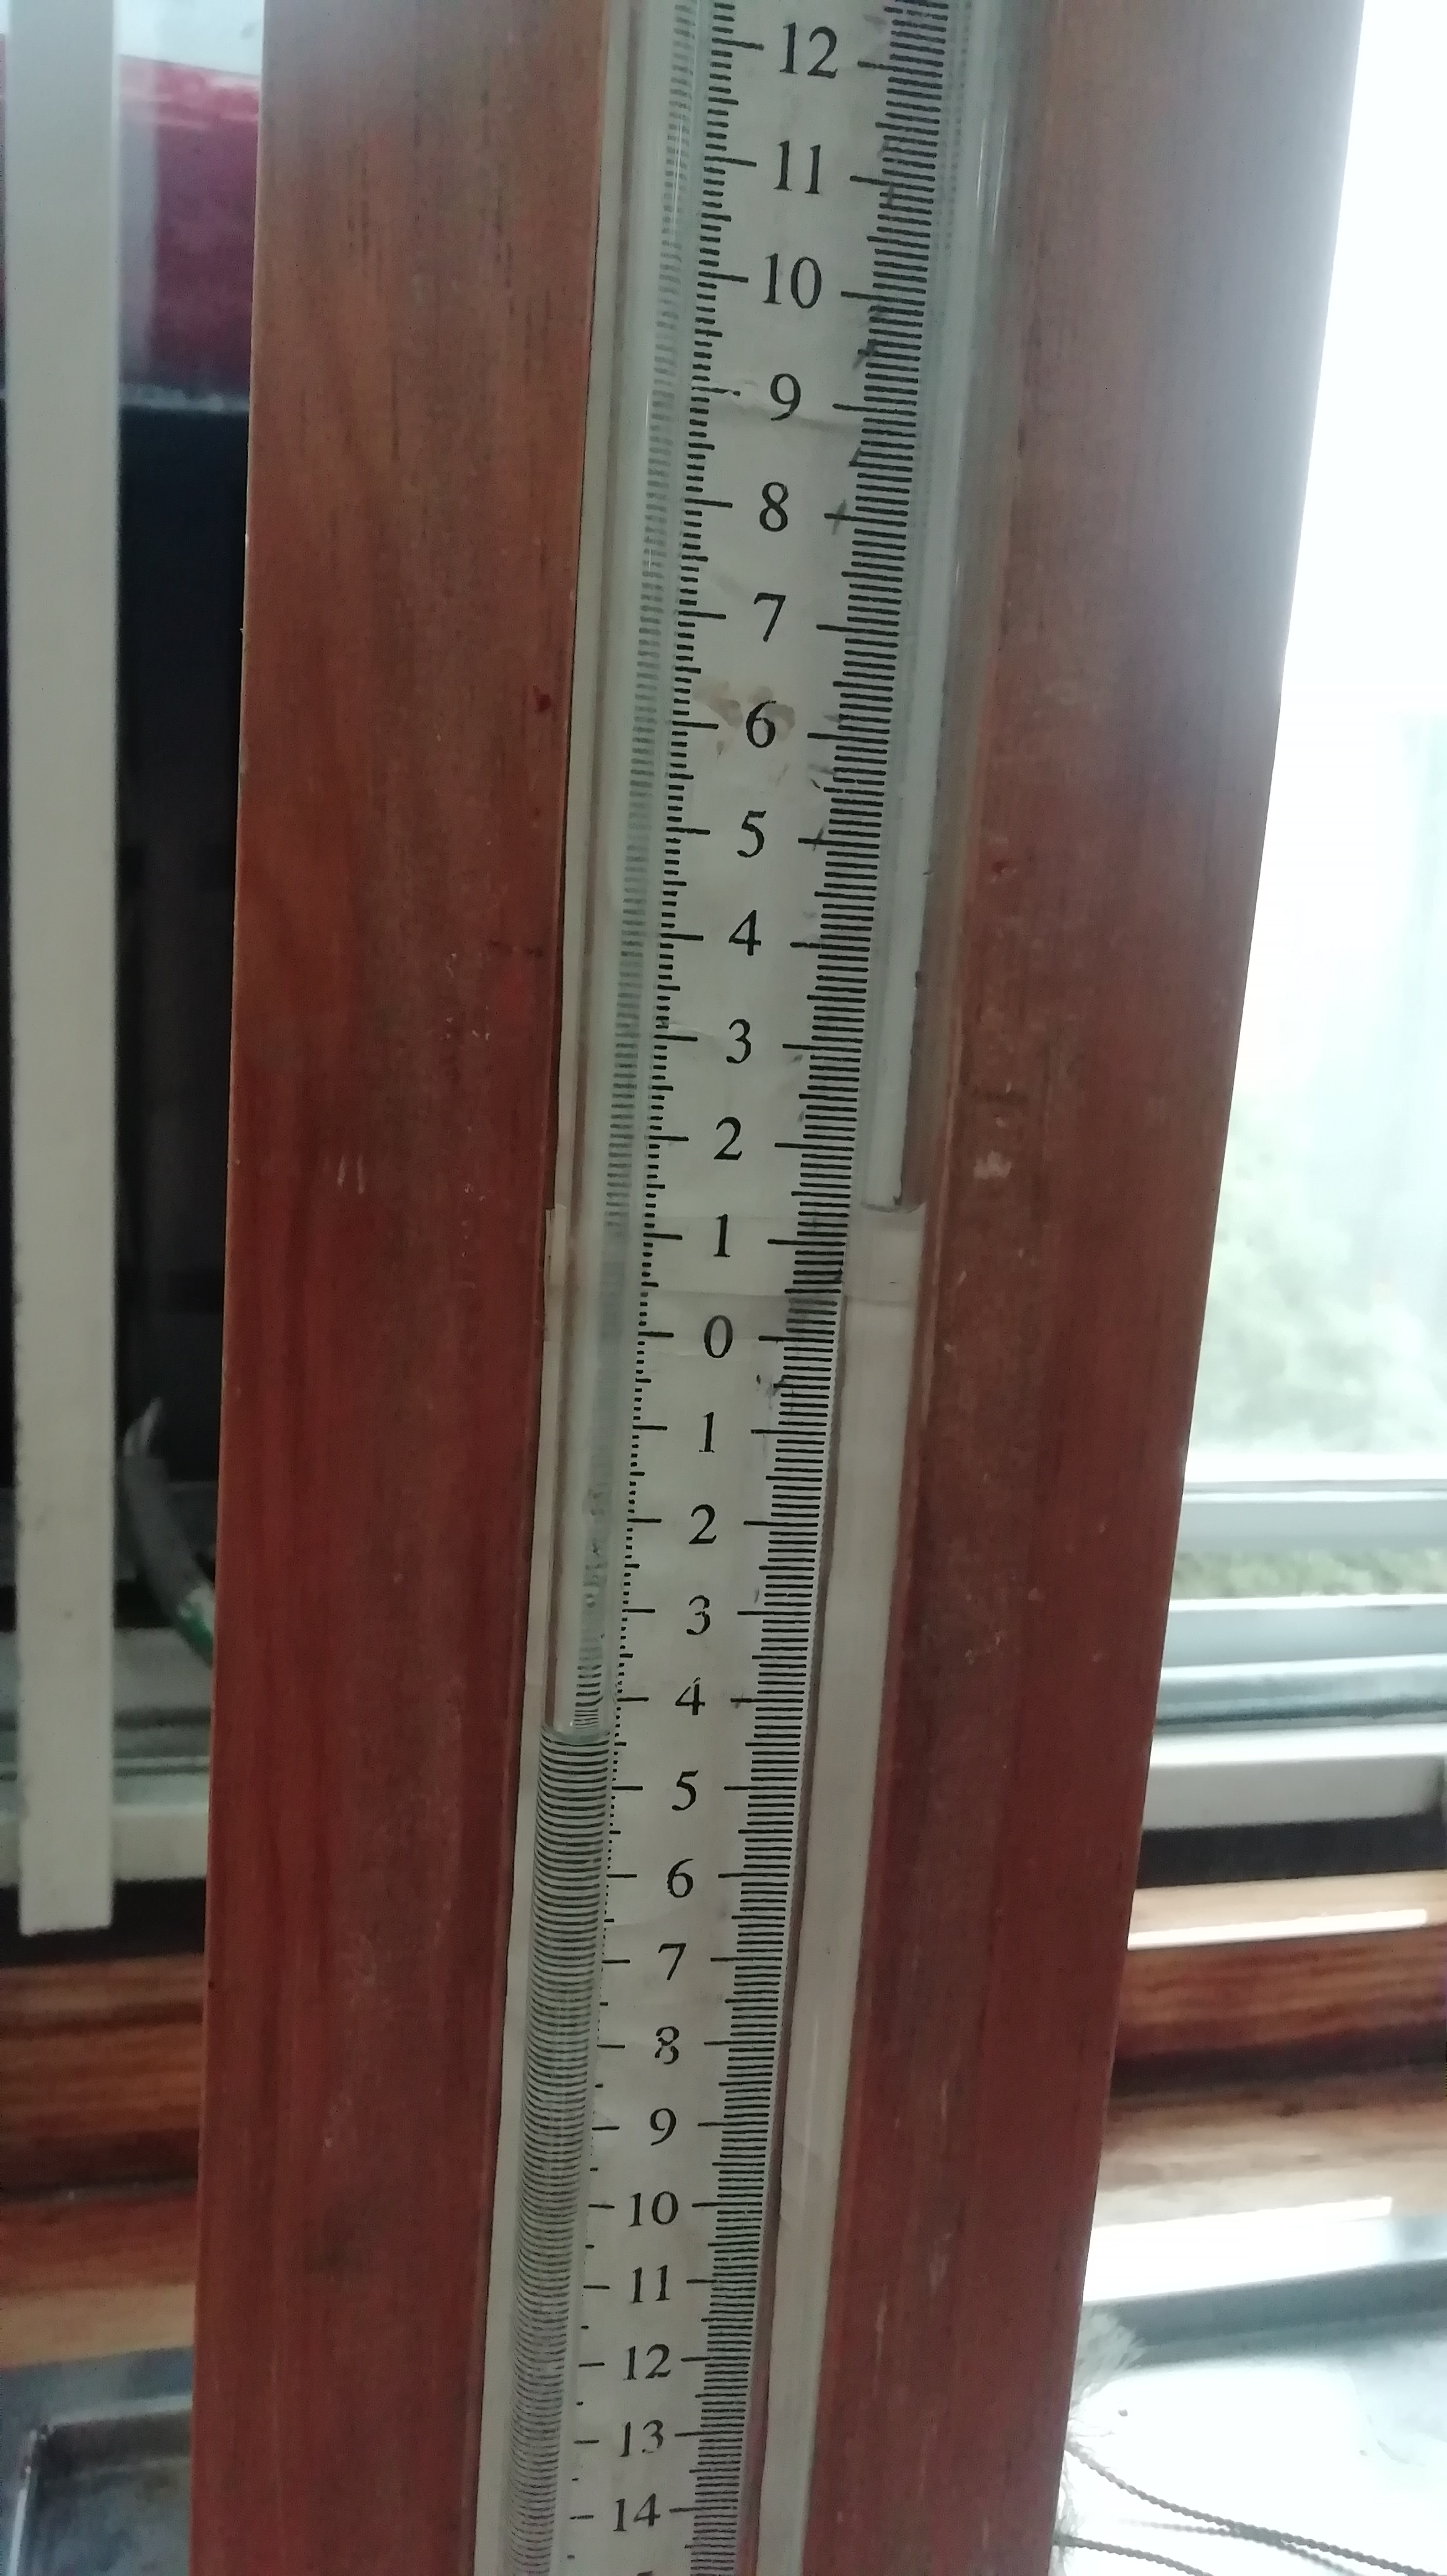
\includegraphics[scale=0.65]{5.png}
\centering
\end{figure}

\begin{figure}[H]
\includegraphics[scale=0.65]{6.png}
\centering
\end{figure}

\begin{figure}[H]
\includegraphics[scale=0.65]{7.png}
\centering
\end{figure}

\begin{figure}[H]
\includegraphics[scale=0.65]{8.png}
\centering
\end{figure}

\begin{figure}[H]
\includegraphics[scale=0.65]{9.png}
\centering
\end{figure}

\begin{figure}[H]
\includegraphics[scale=0.65]{10.png}
\centering
\end{figure}

\begin{figure}[H]
\includegraphics[scale=0.65]{t.png}
\centering
\end{figure}

\begin{figure}[H]
\includegraphics[scale=0.65]{total.png}
\centering
\end{figure}

\newpage
\section{Análisis de resultados.}
\begin{itemize}
    \item Hay una clara tendencia a tener una pendiente menor conforme la tensión se hace más grande.
    \item En cada una de las rectas ajustadas por mínimos cuadrados entre las semilongitudes de onda  y la frecuencia (con tensiones distintas) en todos los casos la xi reducida fue menor a 0.01, lo cual nos menciona un ajuste bastante bueno.
    \item En el caso de la recta ajustada de la tensión y las pendientes, nos proporciona una xi reducida de $8x10^{-6}$, un ajuste muy preciso a una recta.
    \item Claramente en la gráfica de tensión contra las pendientes, se denota una relación inversamente proporcional.
    
\end{itemize}

\section{Conclusiones.}

El objetivo principal de la práctica fue encontrar la relación obtenida entre el número de semilongitudes de ondas (n), la frecuencia (F) y la tensión (T), en un principio encontramos las rectas que mejor se ajustan a la frecuencia contra las semilongitudes, nos dimos cuenta que las tensiones y las pendientes de las rectas obtenidas, tenían una relación inversamente proporcional, lo cual nos permitió poner a la pendiente de las rectas en función de la tensión, así relacionamos las tres variables, como resultado obtuvimos la siguiente relación $n=(-0.0073 \pm 0.0008)TF + (0.083 \pm 0.003)F$.

Como se observó para tensiones más grandes la pendiente de la recta que describe la longitud de onda se vuelve menor, esto se traduce en que si buscamos un mismo número de nodos para dos tensiones distintas no sólo ocurrirá que la frecuencia para cada tensión será distinta sino que para la tensión menor la frecuencia requerida será menor en comparación con las demás. Aunque no se haya podido medir cuantitativamente, podemos ver que ocurre un fenómeno parecido a $ \sqrt{\frac{T}{\mu}} = f \lambda$, de forma que hasta ahora sólo se ha obtenido que $f \propto \frac{T}{n}$ donde $n$ representa el número de semilongitudes; sin embargo, la relación no es precisa, sólo se conoce una relación de dicha forma que es semejante a la que se espera obtener bajo mediciones de otras variables.

Por último, ya que la cuerda no vibra de forma idílica, esto es que vibrara en dos direcciones, fue necesario ignorar y/o mitigar el efecto que este comportamiento causaba sobre las mediciones sin embargo en los resultados se encontraron ajustes con residuos muy pequeños lo cual indica que son muy buenos ajustes que físicamente podemos interpretar en haber encontrado una función que describe de manera casi precisa el comportamiento a estudiar. Es por estos ajustes como se muestra que aunque se hayan ignorado efectos de movimiento en la cuerda estos no afectaron de manera significativa las mediciones.

\begin{thebibliography}{x}

\bibitem{Baz} \textsc{Serway A. }(1997). \textit {Waves. En physics for scientist engineers}. Orlando Florida.

\bibitem{Baz} \textsc{Resnick, Robert }(2001). 
\textit{Movimiento ondulatorio. En Física 1}. México.
\end{thebibliography}
\end{document}